\chapter{Topology of the model and vicinity information}
\label{chapter:vicinity}

In the basic model of minority games all agents act independently without the ability to communicate with each other.
Only means of passing information between them is by using the history of the model that encapsulates all the decisions made by agents in a string of bits.
This simple model allows us to study certain characteristics of competitive systems with limited resources, however it is not a realistic assumption to think of agents as isolated elements that don't communicate with their neighbours.

Once the information of the neighbouring agents is added to the model, two important factors start to influence the dynamics of the system, (i) the dimension of the vicinity, ie. the quantity of neighbouring agents and (ii) the topology of the network generated.

In this chapter we introduce various structures used to model vicinity and how they influence the information flow in the system.
Before diving into vicinity structures, the modifications of the basic model of minority games to include local information is defined in \ref{sec:model modifications}.
First sections, \ref{sec:fixed communities} and \ref{sec:sliding communities}, refer to rather simple structures that are computationally easy to implement and maintain, however they do not express much similarity with real world applications. 
Another similar structure is explained in \ref{sec:von neumann} based on von Neumann distance. 
In the later sections, \ref{sec:scale free}, \ref{sec:small world} and \ref{sec:custom vicinity}, more complex structures are introduced based on graph theory that simulate real world examples more closely. 

\section{Model modifications to include local information}
\label{sec:model modifications}

Once decided to make available new information to agents, we need to decide what that information should be and how will it be used by agents.

Information that we decided to include is the results of reduced minority games consisting of agents in the community.
In addition to global minority game, additional $C$ minority games are added, where $C$ is the number of communities that we want to include.
Each minority game follows the same definitions from Chapter \ref{chapter:minority} and the information generated is available to the agents that define the community. 
Another convention used here is that each minority game contains the same quantity of information available as the global minority game, meaning that if the length of the string of bits representing history is equal to $M$, then also the local history remembered should be $M$ bits long.

To incorporate this change in our basic model the simplest way is to create new kind of agents, called \textit{community agents}, that have the same behaviour, but their brain size is doubled.
By doubling the brain size, we do not have to change the implementation of strategies, only the history that is passed as argument to each strategy. 
For example, a strategy of a new community agent with brain size $2$ is generated is the same fashion as a strategy of a basic agent with brain size $4$ is generated.
A strategy for community agent with brain size $2$ is visible in figure \ref{table:communityStrategy} where first 2 bits, denominated local, are generated by the community minority game of the agent, and second 2 bits, denominated global, are generated by minority game consisting of all the agents.

\begin{table}
\centering
\begin{tabular}{|l|l||l|l| |c|}
\hline
\multicolumn{2}{|c||}{local}&
\multicolumn{2}{|c||}{global}&
\multicolumn{1}{|c|}{prediction} \\
\hline
\hline
0 & 0 & 0 & 1 & 1   \\ \hline
0 & 0 & 1 & 1 & 0   \\ \hline
0 & 1 & 0 & 0 & 0   \\ \hline
0 & 1 & 1 & 1 & 1   \\ \hline
1 & 0 & 0 & 0 & 0   \\ \hline
1 & 0 & 1 & 1 & 0   \\ \hline
1 & 1 & 0 & 0 & 1   \\ \hline
1 & 1 & 1 & 0 & 0   \\ \hline
\end{tabular}
\caption{Example strategy of a community agent with brain size 2}
\label{table:communityStrategy}
\end{table}

One particular case that should be noted is that by dividing the agents in communities, depending on the procedure used, a minority game where the number of agents is pair can occur.
In this case additional guard should be put in the simulation to generate a random winning side when the attendance is equal to $\frac{N}{2}$.
Of course certain procedures are implemented to reduce the number of community minority games with pairwise number of agents to minimum in order to reduce the influence on the whole model. 
Using simple structures this condition does not usually present itself, however when more complex structures are implemented it occurs with higher frequency.
Ad hoc procedures have been implemented in this thesis to reduce the number of pairwise minority games when using scale free and small world structures.

\section{Fixed one-dimensional communities}
\label{sec:fixed communities}

The simplest approach to include local information inside the model is to divide agents in certain number of communities.
By using a one-dimensional list to represent agents we can divide the array in equal parts to model communities.
Let's assume $N$ the number of agents, and $C$ number of communities, the communities are defined as
\begin{displaymath}
C_i = \bigcup agent_j \qquad|\qquad j\in [i, i+\frac{N}{C})
\end{displaymath}
An example division can be seen in figure \ref{fig:fixed vicinity} where a set of $15$ agents is divided in $5$ communities.
When the rest of $\frac{N}{C}$ is different from zero, last $N$ mod $C$ agents are assigned to their own community.

\begin{figure}
\begin{center}
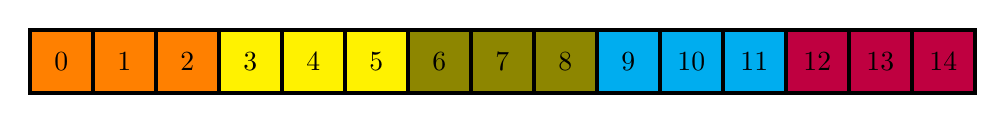
\begin{tikzpicture}[scale=0.8]
\draw [fill=orange,ultra thick] (0,0) rectangle (1,1);
\draw [fill=orange,ultra thick] (1,0) rectangle (2,1);
\draw [fill=orange,ultra thick] (2,0) rectangle (3,1);
\draw [fill=yellow,ultra thick] (3,0) rectangle (4,1);
\draw [fill=yellow,ultra thick] (4,0) rectangle (5,1);
\draw [fill=yellow,ultra thick] (5,0) rectangle (6,1);
\draw [fill=olive,ultra thick] (6,0) rectangle (7,1);
\draw [fill=olive,ultra thick] (7,0) rectangle (8,1);
\draw [fill=olive,ultra thick] (8,0) rectangle (9,1);
\draw [fill=cyan,ultra thick] (9,0) rectangle (10,1);
\draw [fill=cyan,ultra thick] (10,0) rectangle (11,1);
\draw [fill=cyan,ultra thick] (11,0) rectangle (12,1);
\draw [fill=purple,ultra thick] (12,0) rectangle (13,1);
\draw [fill=purple,ultra thick] (13,0) rectangle (14,1);
\draw [fill=purple,ultra thick] (14,0) rectangle (15,1);

\node at (0.5,.5) {0};
\node at (1.5,.5) {1};
\node at (2.5,.5) {2};
\node at (3.5,.5) {3};
\node at (4.5,.5) {4};
\node at (5.5,.5) {5};
\node at (6.5,.5) {6};
\node at (7.5,.5) {7};
\node at (8.5,.5) {8};
\node at (9.5,.5) {9};
\node at (10.5,.5) {10};
\node at (11.5,.5) {11};
\node at (12.5,.5) {12};
\node at (13.5,.5) {13};
\node at (14.5,.5) {14};
\end{tikzpicture}
\caption{Example of 15 agents divided in 5 communities, consisting of 3 agents each}
\label{fig:fixed vicinity}
\end{center}
\end{figure}

This structure creates isolated communities and only way for information to flow between communities is through the global state.
Same local information is available for each agent of the community and it is expected that this information will be used efficiently as they are all involved in the same minority game at a local level. 
However this sort of connectivity between agents does not represent real world examples as in most scenarios communities are not isolated from each other.

\section{Sliding window communities}
\label{sec:sliding communities}

To overcome the difficulty of having isolated communities we take different approach and create a community for each agent.
This is more representative of real world cases and also of the way minority games are defined.

Sliding window technique is used to create communities by creating a local neighbourhood for each agent.
Another possibility opens up here in deciding how many dimension we want to use to represent the set of agents.
We have used one-dimensional arrays and two-dimensional matrix to group agents into communities, and have not delved in higher dimensions as it does not bring any qualitative change, only modifies the graphical representation of agents.

\subsection{Sliding window on one-dimensional array}

Let's assume $N$ is the number of agents and $V$ is an odd integer representing the number of neighbours in each community.
For each agent $a_i$ a community $C_i$ is created from a sliding window of length $V$ centred on agent $a_i$.
an example of this simple procedure can be seen in figure \ref{fig:sliding window one-dimension}

\begin{figure}
\begin{center}
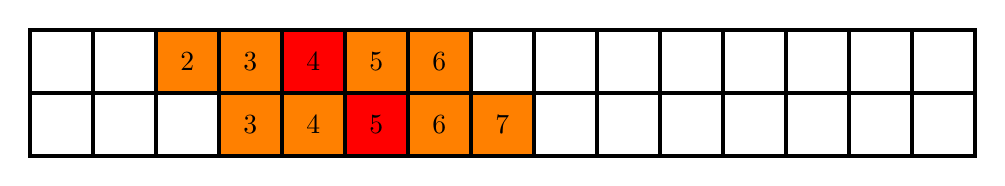
\begin{tikzpicture}[scale=0.8]
\draw [ultra thick] (0,0) rectangle (1,1);
\draw [ultra thick] (1,0) rectangle (2,1);
\draw [ultra thick] (2,0) rectangle (3,1);
\draw [fill=orange,ultra thick] (3,0) rectangle (4,1);
\draw [fill=orange,ultra thick] (4,0) rectangle (5,1);
\draw [fill=red,ultra thick] (5,0) rectangle (6,1);
\draw [fill=orange,ultra thick] (6,0) rectangle (7,1);
\draw [fill=orange,ultra thick] (7,0) rectangle (8,1);
\draw [ultra thick] (8,0) rectangle (9,1);
\draw [ultra thick] (9,0) rectangle (10,1);
\draw [ultra thick] (10,0) rectangle (11,1);
\draw [ultra thick] (11,0) rectangle (12,1);
\draw [ultra thick] (12,0) rectangle (13,1);
\draw [ultra thick] (13,0) rectangle (14,1);
\draw [ultra thick] (14,0) rectangle (15,1);

\draw [ultra thick] (0,1) rectangle (1,2);
\draw [ultra thick] (1,1) rectangle (2,2);
\draw [fill=orange,ultra thick] (2,1) rectangle (3,2);
\draw [fill=orange,ultra thick] (3,1) rectangle (4,2);
\draw [fill=red,ultra thick] (4,1) rectangle (5,2);
\draw [fill=orange,ultra thick] (5,1) rectangle (6,2);
\draw [fill=orange,ultra thick] (6,1) rectangle (7,2);
\draw [ultra thick] (7,1) rectangle (8,2);
\draw [ultra thick] (8,1) rectangle (9,2);
\draw [ultra thick] (9,1) rectangle (10,2);
\draw [ultra thick] (10,1) rectangle (11,2);
\draw [ultra thick] (11,1) rectangle (12,2);
\draw [ultra thick] (12,1) rectangle (13,2);
\draw [ultra thick] (13,1) rectangle (14,2);
\draw [ultra thick] (14,1) rectangle (15,2);

\node at (2.5,1.5) {2};
\node at (3.5,1.5) {3};
\node at (4.5,1.5) {4};
\node at (5.5,1.5) {5};
\node at (6.5,1.5) {6};
\node at (3.5,.5) {3};
\node at (4.5,.5) {4};
\node at (5.5,.5) {5};
\node at (6.5,.5) {6};
\node at (7.5,.5) {7};
\end{tikzpicture}
\caption{Example of communities created using sliding window on one-dimensional array for agents 4 and 5 where each community consists of 5 agents}
\label{fig:sliding window one-dimension}
\end{center}
\end{figure}

\subsection{Sliding window on a matrix}

Different approach is to represent agents in two-dimensional array and construct neighbourhoods on the matrix generated.
This opens possibilities to use different rules for generating the vicinity, such as using the Manhattan distance to generate von Neumann vicinity as described in \ref{sec:von neumann}.
Another simple metric that can be used to generate neighbourhood is Chebyshev distance.
The Chebyshev distance, named after Pafnuty Chebyshev and also called chessboard distance, is defined as a greatest difference of distance along any coordinate dimension between two vectors.

\begin{displaymath}
D_{Chebyshev}(p,q) := max_i (|p_i-q_i|) 
\end{displaymath}

For each agent a community is generated that includes all agents with $D_{Chebyshev}$ less or equal than $R$, where $R$ is the radius of the neighbourhood.

\begin{figure}
        \centering
        \begin{subfigure}[b]{0.3\textwidth}
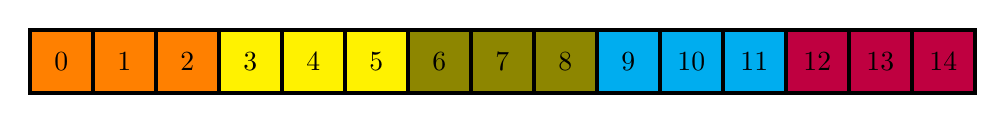
\begin{tikzpicture}[scale=0.8]
\draw [fill=orange,ultra thick] (0,0) rectangle (1,1);
\draw [fill=orange,ultra thick] (1,0) rectangle (2,1);
\draw [fill=orange,ultra thick] (2,0) rectangle (3,1);
\draw [fill=yellow,ultra thick] (3,0) rectangle (4,1);
\draw [fill=yellow,ultra thick] (4,0) rectangle (5,1);
\draw [fill=yellow,ultra thick] (5,0) rectangle (6,1);
\draw [fill=olive,ultra thick] (6,0) rectangle (7,1);
\draw [fill=olive,ultra thick] (7,0) rectangle (8,1);
\draw [fill=olive,ultra thick] (8,0) rectangle (9,1);
\draw [fill=cyan,ultra thick] (9,0) rectangle (10,1);
\draw [fill=cyan,ultra thick] (10,0) rectangle (11,1);
\draw [fill=cyan,ultra thick] (11,0) rectangle (12,1);
\draw [fill=purple,ultra thick] (12,0) rectangle (13,1);
\draw [fill=purple,ultra thick] (13,0) rectangle (14,1);
\draw [fill=purple,ultra thick] (14,0) rectangle (15,1);

\node at (0.5,.5) {0};
\node at (1.5,.5) {1};
\node at (2.5,.5) {2};
\node at (3.5,.5) {3};
\node at (4.5,.5) {4};
\node at (5.5,.5) {5};
\node at (6.5,.5) {6};
\node at (7.5,.5) {7};
\node at (8.5,.5) {8};
\node at (9.5,.5) {9};
\node at (10.5,.5) {10};
\node at (11.5,.5) {11};
\node at (12.5,.5) {12};
\node at (13.5,.5) {13};
\node at (14.5,.5) {14};
\end{tikzpicture}
                \caption{A gull}
                \label{fig:gull}
        \end{subfigure}%
        ~ %add desired spacing between images, e. g. ~, \quad, \qquad, \hfill etc.
          %(or a blank line to force the subfigure onto a new line)
        \begin{subfigure}[b]{0.3\textwidth}
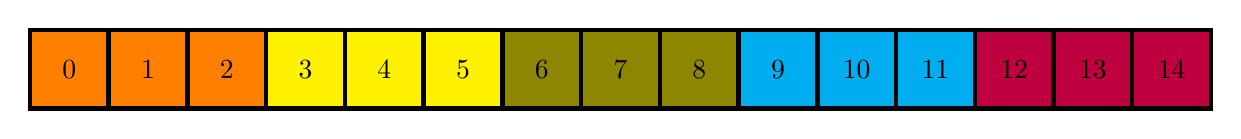
\begin{tikzpicture}
\draw [fill=orange,ultra thick] (0,0) rectangle (1,1);
\draw [fill=orange,ultra thick] (1,0) rectangle (2,1);
\draw [fill=orange,ultra thick] (2,0) rectangle (3,1);
\draw [fill=yellow,ultra thick] (3,0) rectangle (4,1);
\draw [fill=yellow,ultra thick] (4,0) rectangle (5,1);
\draw [fill=yellow,ultra thick] (5,0) rectangle (6,1);
\draw [fill=olive,ultra thick] (6,0) rectangle (7,1);
\draw [fill=olive,ultra thick] (7,0) rectangle (8,1);
\draw [fill=olive,ultra thick] (8,0) rectangle (9,1);
\draw [fill=cyan,ultra thick] (9,0) rectangle (10,1);
\draw [fill=cyan,ultra thick] (10,0) rectangle (11,1);
\draw [fill=cyan,ultra thick] (11,0) rectangle (12,1);
\draw [fill=purple,ultra thick] (12,0) rectangle (13,1);
\draw [fill=purple,ultra thick] (13,0) rectangle (14,1);
\draw [fill=purple,ultra thick] (14,0) rectangle (15,1);

\node at (0.5,.5) {0};
\node at (1.5,.5) {1};
\node at (2.5,.5) {2};
\node at (3.5,.5) {3};
\node at (4.5,.5) {4};
\node at (5.5,.5) {5};
\node at (6.5,.5) {6};
\node at (7.5,.5) {7};
\node at (8.5,.5) {8};
\node at (9.5,.5) {9};
\node at (10.5,.5) {10};
\node at (11.5,.5) {11};
\node at (12.5,.5) {12};
\node at (13.5,.5) {13};
\node at (14.5,.5) {14};
\end{tikzpicture}
                \caption{A tiger}
                \label{fig:tiger}
        \end{subfigure}

        \caption{Pictures of animals}\label{fig:animals}
\end{figure}

\section{Von Neumann Vicinity}
\label{sec:von neumann}

Along with the chessboard metric, Manhattan distance is another option when constructing vicinities.
Called also taxicab distance, this metric is defined as the sum of the lengths of the projections of the line segment between the points onto the coordinate axes.
\begin{displaymath}
d_1(p,q) = ||p-q||_1 = \sum_{i=1}^n |p_i - q_i|
\end{displaymath}



\begin{figure}
        \centering
        \begin{subfigure}[b]{0.4\textwidth}
\centering

\begin{tikzpicture}[scale=0.6]
\foreach \y in {0,...,4}
	\foreach \x in {0,...,4} {
		\ifthenelse{\x=2 \AND \y>0 \AND \y<4}{\def\mycol{orange}}{\def\mycol{white}}
		\ifthenelse{\x=2 \AND \y=2}{\def\mycol{red}}{}
		\ifthenelse{\x=1 \AND \y=2}{\def\mycol{orange}}{}
		\ifthenelse{\x=3 \AND \y=2}{\def\mycol{orange}}{}
		\draw [fill=\mycol](\x, \y) rectangle (\x+1,\y+1);
	}
\end{tikzpicture}
                \caption{Radius 1}
                \label{fig:gull}
        \end{subfigure}
        \begin{subfigure}[b]{0.5\textwidth}
\centering

\begin{tikzpicture}[scale=0.6]
\foreach \y in {0,...,6}
	\foreach \x in {0,...,6} {
		\ifthenelse{\x>1 \AND \x<5 \AND \y>1 \AND \y<5}{\def\mycol{orange}}{\def\mycol{white}}
		\ifthenelse{\x=3 \AND \y=3}{\def\mycol{red}}{}
		\ifthenelse{\x=1 \AND \y=3}{\def\mycol{orange}}{}
		\ifthenelse{\x=3 \AND \y=1}{\def\mycol{orange}}{}
		\ifthenelse{\x=3 \AND \y=5}{\def\mycol{orange}}{}
		\ifthenelse{\x=5 \AND \y=3}{\def\mycol{orange}}{}
		\draw [fill=\mycol](\x, \y) rectangle (\x+1,\y+1);
	}
\end{tikzpicture}
                \caption{Radius 2}
                \label{fig:tiger}
        \end{subfigure}

        \caption{von Neumann vicinity with radius 1 and 2}\label{fig:vonNeumann}
\end{figure}

\section{Scale free network vicinities}
\label{sec:scale free}

\section{Small world network vicinities}
\label{sec:small world}

\section{Custom vicinity structure}
\label{sec:custom vicinity}